%\documentclass[twoside,11pt]{article}
\documentclass[11pt]{article}
\usepackage[natbib, preprint]{jmlr2e}

\usepackage{enumitem}
\usepackage{amsmath}
\usepackage{color}
\usepackage[toc,page]{appendix}
\usepackage{amssymb}
\usepackage{graphicx}
\usepackage{epstopdf}
\usepackage{hyperref}
\usepackage{alltt}
\usepackage{listings}
\usepackage{array}
\usepackage[noline, boxed, linesnumbered, procnumbered, titlenumbered]{algorithm2e}
\usepackage{caption}
\usepackage{subcaption}


\newcommand{\secref}[1]{Section~\ref{#1}}
\newcommand{\appdxref}[1]{Appendix~\ref{#1}}
\newcommand{\tblref}[1]{Table~\ref{#1}}
\newcommand{\figref}[1]{Figure~\ref{#1}}
\newcommand{\thmref}[1]{Theorem~\ref{#1}}
\newcommand{\algref}[1]{Algorithm~\ref{#1}}
\newcommand{\funref}[1]{Function~\ref{#1}}
\newcommand{\eqnref}[1]{Equation~\ref{#1}}
\newcommand{\listingref}[1]{Listing~\ref{#1}}

\newcommand{\eg}{{\em e.g.}}
\newcommand{\ith}{$i^{th}$}
\newcommand{\cut}[1]{}
\newcommand{\todo}[1]{{{\small\color{red}{[#1]}}}}

%\newcommand{\Ex}{\mathop{\mathbb{E}}}
\DeclareMathOperator{\Ex}{\mathbb{E}}

%\newcommand{\Imp}{\mathbf{I}}
\newcommand{\Imp}{\text{Impact}}

\newcommand{\simp}{\fontfamily{cmr}\textsc{\small StratImpact}}
\newcommand{\spd}{\fontfamily{cmr}\textsc{\small StratPD}}
\newcommand{\cspd}{\fontfamily{cmr}\textsc{\small CatStratPD}}
\newcommand{\xnc}{$x_{\overline{c}}$}
\renewcommand{\xi}{x^{(i)}}
\newcommand{\xnC}{$x_{\overline{C}}$}

\setlist[enumerate]{itemsep=-1mm}

% DON'T change margins - should be 1 inch all around.
\cut{
\addtolength{\oddsidemargin}{-.5in}%
\addtolength{\evensidemargin}{-.5in}%
\addtolength{\textwidth}{1in}%
\addtolength{\textheight}{1.3in}%
\addtolength{\topmargin}{-.8in}%
}

\ShortHeadings{Tech Report: Model-Free Feature Impact and Importance}{Parr, Wilson, and Hamrick}
\firstpageno{1}

\begin{document}

\def\spacingset#1{\renewcommand{\baselinestretch}%
{#1}\small\normalsize} \spacingset{1}


%%%%%%%%%%%%%%%%%%%%%%%%%%%%%%%%%%%%%%%%%%%%%%%%%%%%%%%%%%%%%%%%%%%%%%%%%%%%%%

\title{\bf Tech Report: Model-Free Feature Impact and Importance}

\author{Terence Parr \email parrt@cs.usfca.edu
\addr University of San Francisco\\
\AND James D. Wilson \email jdwilson4@usfca.edu
\addr University of San Francisco\\
\AND Jeff Hamrick \email jhamrick@usfca.edu
      \addr University of San Francisco}

\maketitle

\begin{abstract}%
Practitioners use feature importance to rank and eliminate weak predictors during model development in an effort to simplify models and improve generality.  Unfortunately, they also routinely conflate such feature importance measures with feature impact, the isolated effect of an explanatory variable on the response variable.   This can lead to real-world consequences when importance is inappropriately interpreted as impact for business or medical insight purposes. The dominant approach for computing importances is through interrogation of a fitted model, which works well for feature selection, but gives distorted measures of feature impact. The same technique applied to the same data set can yield different feature importances, depending on the model, leading us to conclude that impact should be computed directly from the data.  While there are model-free feature selection algorithms, they typically yield just feature rankings, rather than measures of impact or importance. In this paper, we give mathematical definitions of feature impact and importance that operate directly on the data and, to assess their quality, show that features ranked by these definitions are competitive with existing techniques for feature selection using three real data sets. \todo{should we reference shap, permutation importance, mRMR in abstract?}
\end{abstract}

\begin{keywords}
feature importance, business insights, medical insights, partial dependence, model interpretability, machine learning
\end{keywords}

\section{Introduction}
\label{sec:intro}

Among data analysis techniques, feature importance is one of the most widely applied and practitioners use it for two key purposes. First, to select features for predictive models (dropping the least predictive features to simplify and potentially increase the generality of the model). Second, to gain business or medical insights, such as identifying product characteristics valued by customers or treatments contributing to patient recovery.  To distinguish the two use cases, we will refer to feature predictiveness for modeling purposes as {\em importance} (the usual meaning) and the effect of features on business or medical response variables as {\em impact}.

While some feature importance approaches work directly on the data, such as minimal-redundancy-maximal-relevance (mRMR) by \cite{mRMR}, almost all algorithms used in practice rank features by interrogating a specific fitted model (e.g., SHAP by \citealt{shap}, permutation importance by \citealt{RF}, and drop column importance), or even interrogating subsidiary models to analyze such fitted models (e.g., LIME by \citealt{lime}). It is accepted as self-evident that identifying the most important features for a model is best done through interrogation of that  model, but this is not always the case.  For example, when asked to identify the single most important feature of a real dataset \citep{bulldozer}, through interrogation and validation on a random forest, the features selected by model-based techniques get twice the validation error of the model-free technique proposed in this paper; see \figref{fig:topk}(c). Still, model interrogation is generally effective in practice for feature importance purposes. (In our experience, it is best to get importances using multiple techniques and to view the combined results as a clue rather than the gospel truth.)

Feature importance should not, however, be interpreted as feature impact for several reasons. First, predictive features do not always coincide with impactful features; e.g., models unable to capture complex nonlinear feature-response relationships rank such features as unimportant, even if they have large impacts on the response. Next, practitioners must develop models accurate enough to yield meaningful feature importances, but there is no definition of ``accurate enough.'' Finally, it is possible to get very different feature importances (and hence impacts) running the same algorithm on the same data, just by choosing a different model. This is despite the fact that true feature impacts are relationships that exist in the data, with or without a model.

Consider the feature importance charts in \figref{fig:diff-models} derived from four different models on the same, well-known Boston toy data set, as computed by SHAP that has recently emerged as the front runner in feature importance. The linear model (a) struggles to capture the relationship between features and response variable ($R^2$=0.74), so those importances are less trustworthy.  In contrast, the random forest (b), boosted trees (c), and support vector machine (d) models capture the relationship in the training records (all 506) with high fidelity, but SHAP derives meaningfully different feature importances from each model. The differences arise because feature importances are distorted by the lens' of the models, making it unclear which ranking, if any, gives the true feature impacts. 

\begin{figure}[htbp]
\begin{center}
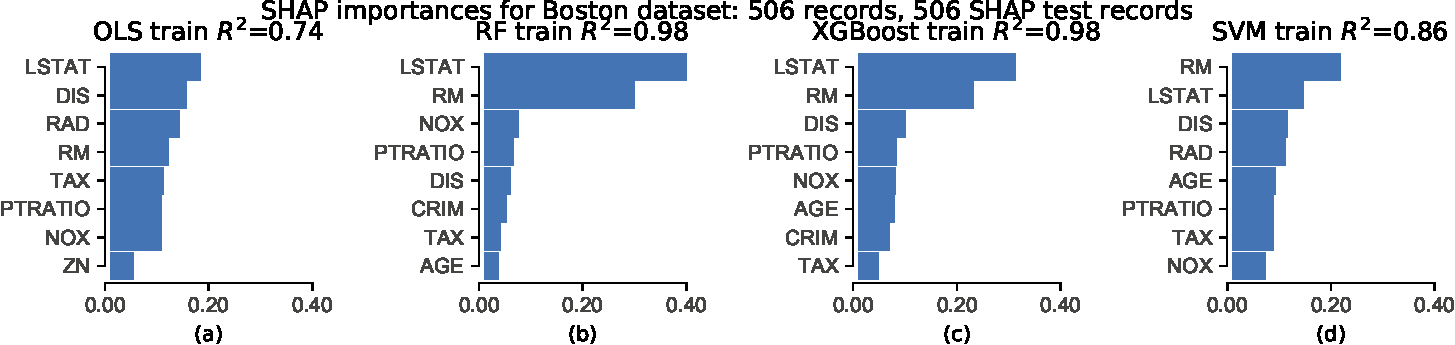
\includegraphics[scale=0.6]{images/diff-models.pdf}
\caption{\small Ranking and relative predictiveness of the top 8 of 13 Boston data set features determined by SHAP interrogating four different models.  There is considerable variation, particularly for the random forest (RF) model and we chose a random seed to highlight the possibility of conflicting results from the same technique applied to the same data. Rough timing for explaining $n$=506 test records is (a) less than 1 second, (b) 10s, (c) 3s, and (d) 13 minutes.  Scikit-learn model hyper-parameters: OLS normalized explanatory variables; RF with 30 trees; XGBoost with 50 trees, $\eta=0.01$, max depth 5; SVM with $\gamma=0.001$, $C=100$.}
\label{fig:diff-models}
\end{center}
\end{figure}

Unfortunately, practitioners routinely conflate model-based feature importance with impact and have, consequently, likely made business or medical decisions based upon faulty information. Despite the potentially serious real-world consequences resulting from inappropriate application of importances, research attention has focused primarily on feature importance rather than impact. 

In this paper, we address this deficiency by contributing (1) a simple mathematical formula for computing feature impact that is purely a function of the training data, rather than a fitted model  provided by the user, and (2) an efficient implementation called \simp{} that yields plausible feature impacts.   In order to measure the quality of feature impacts, we observe that features with the most impact on the response variable should coincide with the most predictive features, particularly if variable density among the validation records is taken into consideration. We, therefore, define feature importance as a weighted variation of feature impact. Using impact-derived importances as a proxy for impacts, our experiments on real data show that \simp{} is competitive with existing importance techniques, as measured by cross-validation errors on models trained using the top importances.   We emphasize that these impact and importance definitions are insensitive to codependencies among features and apply to both numerical and categorical features.  (The latter is essential because virtually all real-world datasets have categorical variables.) While we focus solely on regression here, a similar approach would work for classification.

We begin by giving definitions of feature impact and importance in \secref{sec:def}, then survey  existing model-free and model-dependent techniques in \secref{sec:existing}. \secref{sec:experiments} assesses the quality of \simp{} impact values by measuring their effectiveness as feature rankings. We finish in \secref{sec:discussion} with a discussion of the proposed technique's effectiveness, prototype implementation's performance, and future work.

\section{Mathematical definitions of impact and importance}\label{sec:def}

\cut{Practitioners loosely define feature importance as feature predictiveness, which presupposes a fitted predictive model, probably because importances are so often used for feature selection during model development.  Research  focuses on more accurately identifying the impact of features upon model predictions.  But, relying on a fitted model makes it difficult to tease apart the true feature importance from the ability of the model to exploit that feature for prediction purposes. Rather than measuring feature impact on {\em model predictions}, we propose avoiding the model completely to define feature importance as the average impact of a feature on the {\em data set response values}.}

In special circumstances, we know the precise impact of each feature $x_j$. Assume we are given training data pair ($\bf X, y$) where ${\bf X} = [x^{(1)}, \ldots, x^{(n)}]$ is an $n \times p$ matrix whose $p$ columns represent observed features and ${\bf y}$ is the $n \times 1$ vector of responses.  If a data set is generated using a linear function, $y = \beta_0 + \sum_{j=1}^p \beta_j x_j$, \todo{assumes independence of $x_j$? I don't think so since we have complete equation} then coefficient $\beta_j$ corresponds exactly to the impact of $x_j$.  $\beta_j$ is the impact on $y$ for a unit change in $x_j$, holding all other features constant.

To hold features constant for any smooth generator function, we can take the partial derivatives of $y$ with respect to each feature $x_j$. For any smooth function $f:\mathbb{R}^{p} \rightarrow \mathbb{R}$ that precisely maps each $\xi$ to $y^{(i)}$, ${y^{(i)}} = f(\xi)$, the partial derivative of $y$ with respect to $x_j$ gives the change in $y$ holding all other variables constant; e.g., for linear functions, $\frac{\partial y}{\partial x_j}=\beta_j$. Integrating the partial derivative then gives the {\em partial dependence}  of $y$ on $x_j$, the isolated contribution of $x_j$ to $y$. But, rather than relying on a fitted model as originally formulated by \citep{PDP}, this definition of partial dependence relies on the partial derivative of a known function that generated the data set.

~\\
\noindent {\bf Definition 1} The {\em model-free partial dependence} of $y$ on feature $x_j$ for smooth generator function $f:\mathbb{R}^{p} \rightarrow \mathbb{R}$ evaluated at $x_j = z$ is the cumulative sum up to $z$:

\begin{equation}\label{eq:pd}
\text{\it PD}_j(z) = \int_{min(x_j)}^z \frac{\partial y}{\partial x_j} dx_j
\end{equation}

\todo{This is zeroed to have the y-intercept removed  whereas the normal definition does not, SHAP is doing a "centered ICE plot" version where the anchor point is $\bar{y}$}

$\text{\it PD}_j(z)$ is the value contributed to $y$ by $x_j$ at $x_j = z$. The advantages of this partial dependence definition are that it does not depend on a fitted model and is insensitive to collinear or otherwise codependent features, unlike the traditional definition that is accurate for data ``{\em dominated by low order interactions}'' per Friedman.  \todo{use FPD for friedman as differs from our PD} 

To go from partial dependence to feature impact, we compare the area under the absolute value of each partial dependence curve. The larger the area under the curve, the larger the impact on $y$.   By the mean-value theorem of integrals, the area under $f(x)$ in interval $[a,b]$ is $\int_{a}^{b} f(x) dx = \overline{f(x)}(b-a)$.  For comparison purposes between variables, the actual area is not important and the $b-a$ term drops out, assuming the variables our normalized so all $x_j$ domains have the same range, such as $[0,1]$. The impact of $x_j$ is then just the average magnitude of $\text{\it PD}_j(x_j)$:

~\\
\noindent {\bf Definition 2} The feature impact of $x_j$ is the ratio of $x_j$'s average partial dependence magnitude to the total for all variables, when all $x_j$ variables are normalized to the same fixed range:

\begin{equation}\label{eq:Epd2a}
\Imp_j = \frac{\overline{|\text{\it PD}_j|}}{\sum_{k=1}^p \overline{|\text{\it PD}_k|}}
\end{equation}

\todo{even if we had perfect PD, I'm not sure the following is true unless we get rid of the absolute value operators: $\overline{|y|} = \sum_{k=1}^p \overline{|\text{\it PD}_k|}$, meaning we cannot simplify the denominator for impact}


\noindent For example, consider quadratic equation $y = x_1^2 + x_2 + 100$ as a generator of data in $[0,3]$. The partial derivatives are $\frac{\partial y}{\partial x_1} = 2 x_1$ and $\frac{\partial y}{\partial x_2} = 1$, giving $\text{\it PD}_1 = x_1^2$ and $\text{\it PD}_2 = x_2$. $\overline{|\text{\it PD}_1|}$ is then 9.0, the average magnitude of $x_1^2$ in $[0,3]$, and $\overline{|\text{\it PD}_2|}$ is 4.5, the average magnitude of $x_2$ in $[0,3]$, as depicted in \figref{fig:quad-area}(a). That is the same result obtained by integrating under the partial dependence curves:  $\int_0^3 x_1^2 dx_1 = \frac{x_1^3}{3} \big |_0^3 = 9$ and $\int_0^3 x_2^2 dx_2 = \frac{x_2^2}{2} \big |_0^3 = 4.5$.   Therefore, $x_1$ has twice the impact as $x_2$ for data generated in that interval, giving $\Imp_1 = 0.\overline{66}$ and $\Imp_2 = 0.\overline{33}$.


\begin{figure}[htbp]
\begin{center}
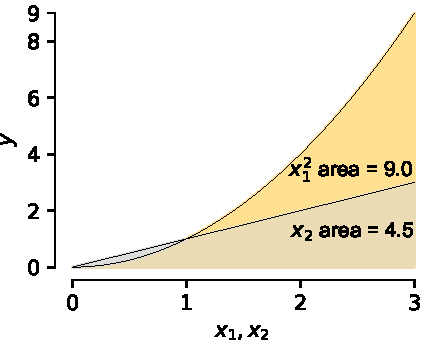
\includegraphics[scale=0.6]{images/quadratic-auc.pdf}
\captionof{figure}{\small  (a) The area under $x_1$ and $x_2$ partial dependence curves represent $\Imp_1$, $\Imp_2$ for $y = x_1^2 + x_2 + 100$ in range $[0,3]$. Figures (b) and (c) illustrate the difference between the area straddling the mean and the area under the partial dependence curve. Simulation of $n$=2,000 records: 10 trials of \simp{} gives impact (area-under-curve) for (b) and (c) as $x_1$ = 3.1739 ($\sigma=0.047$) and $x_2$ = 1.4696 ($\sigma=0.005$); SHAP gives impact as $x_1$ = 7.0812 and $x_2$ = 2.2108 (which were multiplied by the range of 3 to get area). These simulated area values coincide closely with the true areas under the curve (\simp) and areas straddling the $x_j$ means (SHAP).}
\label{fig:quad-area}
\end{center}
\end{figure}

The obvious disadvantage of this feature impact definition is that function $f$, from which $\text{\it PD}_j$ is derived, is unknown in practice, so symbolically computing the partial derivatives is not possible. But, if we could compute accurate partial dependence curves by some other method, then this definition would still represent a viable means to obtain feature impacts. 

As originally defined, partial dependence curves are derived from fitted models and are biased in the presence of codependent variables.  To overcome this bias and to avoid the need for predictions from a fitted model, we recently introduced a technique called \spd{} (\citealt{stratpd}) to approximate partial dependence curves using a data stratification approach. \spd{} stratifies a data set into groups of observations that are similar, except in the variable of interest, $x_j$, through the use of a single decision tree. Any fluctuation of the response variable within a group (decision tree leaf) is likely due to $x_j$. The $\beta_1$ coefficient of a simple local linear regression fit to the $(x_j, y)$ values within a group provides an estimate of $\frac{\partial y}{\partial x_j}$ in that group's $x_j$ range. Averaging the partial derivative estimates across all such groups yields the overall $\frac{\partial y}{\partial x_j}$ partial derivative approximation. The cumulative sum of the estimated partial derivative yields the partial dependence curve. 

For categorical variables, \cspd{} uses the same stratification approach, but cannot apply  regression of $y$ on categorical $x_j$. Instead, a random reference category is chosen for each group and its $y$ value is subtracted from all leaf $y$ to get relative impacts between categories. The relative category impacts across groups are then averaged to get the impact of each $x_j$ on $y$.  (Note that \cspd{} and \spd{} never use predictions from any model---they use decision trees merely to stratify feature space and \spd{} uses piecewise linear regressors just to get slope estimates.)

\cut{
\begin{figure}[htbp]
\begin{center}
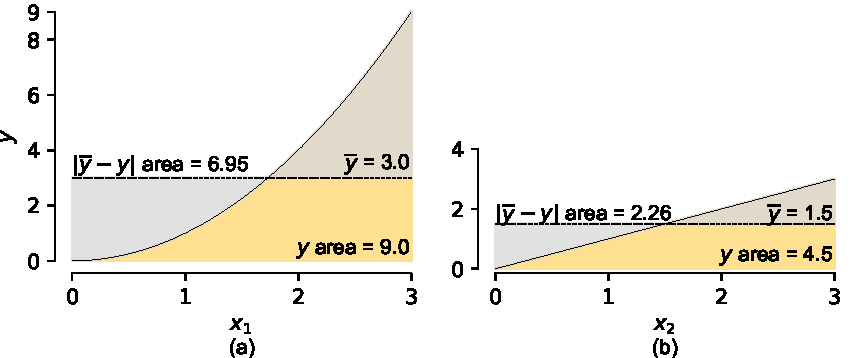
\includegraphics[scale=0.65]{images/from-mean-auc.pdf}
\captionof{figure}{AUC for partial dependence curves from $y = x_1^2 + x_2 + 100$ in $[0,3]$ Shows why must compute from 0 not deviation from mean}
\label{fig:combined-area}
\end{center}
\end{figure}
}

Intuitively, the impact of $x_j$ is how much, on average, the values of $x_j$ are expected to push $y$ away from zero. We deliberately chose this  definition instead of measuring how much $x_j$ pushes $y$ away from the average response, $\overline{y}$. The impact of $x_1$ on $y$ is $x_1^2$, not $\overline{y} - x_1^2$; $\overline{y}$ has contributions from all $x_j$  For example, at $x_j=0$, the impact on $y$ should be 0, not $\overline{y}-0 = \overline{y}$.  \figref{fig:quad-area}(b) and \figref{fig:quad-area}(c) illustrate how the area under the $x_1^2$ and $x_2$ partial dependence curves from $y = x_1^2+x_2+100$ differ from the area straddling the means. The true area under-the-curve ratio of $x_1$-to-$x_2$ is 2-to-1 (9/4.5), whereas the ratio of the area straddling the mean has roughly a 3-to-1 ratio (6.95/2.26).

\begin{figure}[htbp]
\begin{center}
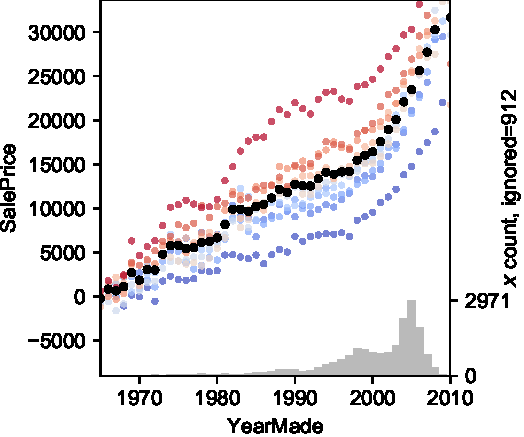
\includegraphics[scale=0.5]{images/bulldozer-YearMade.pdf}
\captionof{figure}{\small The partial dependence of {\tt SalePrice} on feature {\tt YearMade} for the bulldozer data set including the feature histogram used to weight the partial dependence to obtain feature importances; this plot represents a 20k subsample of 363k records.}
\label{fig:yearmade}
\end{center}
\end{figure}

For business or medical insight purposes, deriving feature impacts from partial dependence curves make sense because these curves describe how each $x_j$ value found in the data set effects $y$. When selecting features for modeling, however, feature impact values should take $x_j$ density into consideration. Model validation error is sensitive to the distribution of the records in the validation set, not just the selection of most impactful features.  For example, \figref{fig:yearmade} shows the partial dependence curve for feature {\tt\small YearMade} and the histogram of $x_j$ values from the bulldozer auction data set \citep{bulldozer}; the colored curves represent ten bootstrapped data sets and the black dots give the average curve.  Knowing that increased bulldozer age continues to reduce price is useful from a business perspective, but the bulk of the validation set will have newer bulldozers.  This leads to a feature importance definition based upon expected value of the partial dependence magnitude rather than simple averages across $x_j$ domains.

\cut{
While feature importances should not be interpreted as feature impacts, impacts can be effective as feature importances for model feature selection.  Features with the most impact on the response variable the most should coincide with the most predictive features. But, m

The definition of impact in \eqnref{eq:Epd2a} assumes that each $x_j$ value is equally likely, which is not the case in practice for $(\bf X, y)$ data sets. To go from partial dependence to importance, the $\text{\it PD}_j$ curve at $x_j=z$ must be weighted by the number of samples at $x_j=z$ before computing the average magnitude.  The red dots represent the $\text{\it PD}_j$ weighted according to the histogram height and the orange region represents the impact {\tt\small YearMade} has on the response variable, {\tt\small SalePrice}. While the {\tt\small YearMade} partial dependence curve is plausible before year 1990 (older bulldozers are worth less), there are so few data points that the collection of very old bulldozers should have little overall effect on the overall average sale price.  This leads to a definition based upon expected value rather than simple averages across $x_j$ domains.
}

~\\
\noindent {\bf Definition 3} The {\em model-free feature importance} of $x_j$ is the ratio of $x_j$'s expected partial dependence value to the total of all expected values, when all $x_j$ variables are normalized to the same fixed range:

\begin{equation}\label{eq:Epd2b}
\text{Importance}_j = \frac{\Ex[|\text{\it PD}_j|]}{\sum_{k=1}^p \Ex[|\text{\it PD}_k|]}
\end{equation}

\noindent where:

\begin{equation}\label{eq:Epd2c}
\Ex[|\text{\it PD}_j|] = \frac{1}{n} \sum_{i=1}^{n} |x_j[x_j=x_j^{(i)}]| \times  |\text{\it PD}_j(x_j^{(i)})|
\end{equation}

\noindent with $x_j[x_j=x_j^{(i)}]$ denoting the count of $x_j$ values equal to $x_j^{(i)}$.

\section{Existing methods}\label{sec:existing}

In this paper, we are primarily concerned with identifying the most impactful features for business or medical applications. But, because virtually all research focuses on feature importance and because practitioners commonly assume feature importance is the same as feature impact, it is appropriate to compare \simp{} to  feature importance methods.

Feature importance methods for labeled data sets (with $\bf X$ and $\bf y$) are broadly categorized into data analysis and model analysis techniques, sometimes called {\em filter} and {\em wrapper} methods \citep{tsanas}. Data analysis techniques analyze the data directly to identify important features, whereas model analysis techniques rely on predictions from fitted models.  The data analysis techniques further split into techniques for regression and techniques for classification, with most of the research going into classification.

The simplest technique to identify important or relevant regression features is to rank them by their Spearman's rank correlation coefficient \citep{spearmans}; the feature with the largest coefficient is taken to be the most important. This method works well for independent features, but suffers in the presence of codependent features.   Groups of features with similar relationships to the response variable receive the same or similar ranks, even though just one should be considered important.

Another possibility is to use principle component analysis (PCA), which operates on just the $\bf X$ explanatory matrix. PCA transforms data into a new space characterized by eigenvectors and identifies features that explain the most variance in the new space. If the first principal component covers a large percentage of the variance, the ``loads'' associated with that component can indicate importance of features in the original $\bf X$ space. PCA is limited to linear relationships, however, and ``most variation'' is not always the same thing as ``most important.''

For classification data sets, the Relief algorithm \citep{relief} tries to identify features that distinguish between classes through repeated sampling of the data. For a sampled observation $\xi$, the algorithm finds the nearest observation with the same class (hit) and the nearest observation with the other class (miss). The score of each attribute, $x_j$, is then updated according to the distance from the selected $\xi$ to the hit and miss observations'  $x_j$ values. ReliefF \citep{ReliefF} extended Relief to work on multiclass problems and RReliefF \citep{RReliefF} adapted the technique to regression problems (by ``...introduc[ing] a kind of probability that the predicted values of two instances are different'').

In an effort to deal with codependencies, data analysis techniques rank features not just by {\em relevance} (correlation with the response variable) but also by low {\em redundancy}, the amount of information shared between codependent features, which is the idea behind minimal-redundancy-maximal-relevance (mRMR) by \citep{mRMR}. mRMR selects features in order according to the following score.

\[
J_{mRMR}(x_k) = I(x_k, y) - \frac{1}{|S|} \sum_{x_k \in S} I(x_k, x_j)
\]

\noindent where $I(x_k, x_j)$ is some measure of mutual information between $x_k$ and $x_j$, $S$ is the growing set of selected features, and $x_k$ is the candidate feature. mRMR only considers single-feature relationships with the response variable, and is limited to classification as originally defined. See \citep{ubermRMR} for a recent application of mRMR at Uber Technologies.  For more on model-free feature importances, see the survey by \citep{survey}.  \citet{tsanas} suggests using spearman's rank not mutual information. \citet{meyer-microarray} looks for pairs of features to response variable associations as an improvement, while retaining reasonable efficiency. See \citet{filter-benchmark} for benchmarks of filter versus filter methods.

The fundamental problem faced by all of these data analysis techniques is that they measure relevance by the strength of the association between (typically) a single feature to response $y$, but $y$ contains the impact of all $x_j$ variables. Computing an appropriate association metric between categorical and numeric values also presents a challenge.  In contrast, the definitions of impact and importance proposed in this paper isolate the effect of each $x_j$ on $y$, holding all other variables constant, and also support categorical features.
 
Turning to model-based techniques, feature importance methods are typically variations on a theme: tweak the model and measure the effect on model prediction accuracy or expected model output. The simplest approach is {\em drop-column importance}, which defines $x_j$ importance as the difference in model accuracy between a model with all features (the baseline) and a model with $x_j$ removed. The model must be retrained $p$ times and highly similar features yield low or zero importances because codependent features cover for the dropped column in the model.

To avoid retraining the model, $x_j$ can be permuted instead of dropped for {\em permutation importance}. This approach is faster but can introduce nonsensical observations by permuting invalid values into records; e.g., shifting a true {\tt\small pregnant} value into a male's record. Codependent features tend to share importance, at least when permutation importance is applied to random forest models.

Rather than removing or permuting entire columns of data, LIME \citep{lime} and SHAP \citep{shap} focus on model behavior at the observation level. For a feature vector of interest, LIME trains an interpretable linear model, on a small neighborhood of data around that vector to explain the relationship between variables and the response locally. SHAP, however, was shown to subsume the LIME technique in \citep{shap}. 

SHAP has its roots in {\em Shapley regression values} \citep{shapley-regression} where (linear) models were trained on all possible subsets of features.  Each possible model pair differing in a single feature $x_j$ contributed the difference in model pair output towards the Shapley value for $x_j$. The complete Shapley value is the average model-pair difference weighted by the number of possible pairs differing in just $x_j$. This technique isolates the effect of $x_j$ on $y$ well, but through the lens of a model, so Shapley values should be interpreted as feature importances not feature impacts. For completely independent features, drop-column importance is sufficient because the contribution of $x_j$ can be computed without considering how combinations of features affect model output.  In practice, features are rarely independent and the marginal effect of adding a new feature on model output depends on the order in which features are added.  

To avoid training a combinatorial explosion of models with the various feature subsets, $\hat{f}_S(x_S)$, SHAP reuses the same fitted model by running simplified feature vectors into the model. One possible implementation for simplified vectors is to replace ``missing'' $x_j$ features with the expected value of $x_j$. Instead, SHAP's implementation approximates $\hat{f}_S(x_S)$, with $\Ex[\hat{f}(x_{S},{\bf X}_{\bar{S}}) | {\bf X}_S = x_S]$ then further approximates with $\Ex[\hat{f}(x_{S},{\bf X}_{\bar{S}})]$ by assuming feature independence. \cite{janzing2019feature} argues that ``{\em unconditional} [emphasis theirs] rather than {\em conditional} expectations provide the right notion of dropping features.''  SHAP engages this behavior in ``interventional'' mode, and users can pass in a so-called {\em background set} that contains, for example, $x_j$ averages or even the entire $\bf X$ training set. To further reduce computation costs, SHAP users typically compute values for a very small subsample of the data set, with the commensurate reduction in explanatory precision of the underlying population. SHAP has model-type-dependent optimizations for linear regression, deep learning, and decision-tree based models.

While SHAP has very strong theoretical foundations, we cannot agree with the formal SHAP definition of feature impact for the simple reason that SHAP measures $x_j$ impact as the magnitude of the deviations $x_j$ causes from the mean model prediction, $\overline{y}$, rather than deviations from $y=0$.   For example, given equation $y=x_1^2 + x_2 + 100$ from \figref{fig:quad-area}, the effect of $x_1$ on $y$ is clearly $x_1^2$ (whose impact is the area of the orange region), not $|\overline{y} - x_1^2|$, as defined by SHAP (grey region area). 

The formal SHAP definition does not assume feature independence as the implementation does, leading to further problems

\begin{theorem}
The average of the SHAP values at any $x_j=z$ location estimates the mean-centered FPD partial dependence curve, assuming independent features: $\Ex[ \phi_j(\hat{f},x) | {\bf X}_j = z] = FPD_j(x) - \bar{y}$.
\end{theorem}



We also see several practical SHAP disadvantages:

\begin{itemize}
\item  For performance reasons, SHAP effectively limits the user's choice of model to those with model-type-dependent implementations, such as {\tt\small TreeExplainer}; e.g., SHAP applied to a support vector machine trained on Boston's 506 records takes 13 minutes to explain the same 506 records.  Large data sets also pose problems even for the model-type-dependent optimizations; e.g., SHAP applied to a modest 50-tree random forest trained on 1.2M record ``League of legends'' data set \citep{lol} takes 25 minutes to process a sample of size 1000.

\item As with permutation methods, replacing feature values with their expectations or a random selection introduces the possibility of creating nonsensical feature vectors.  For example, replacing the bulldozer {\tt\small YearMade} feature with the overall {\tt\small YearMade} average, risks conjuring up a type of bulldozer that did not exist in that year. This biases the feature contribution estimates.

\item SHAP documentation claims to break ``the dependencies between features according to the rules dictated by casual inference'' citing \citet{janzing2019feature}, but we find that SHAP ``interventional'' mode is still unable to disentangle codependent features for a synthetic body weight data set with codependent {\tt\small sex}/{\tt\small pregnant}/{\tt\small height} features (Equation (7) from \citealt{stratpd}):

\begin{equation}\label{eq:weight}
y_{weight}  = 120 + 10(x_{height} - min(x_{height})) + 70x_{pregnant} - 1.5x_{education}
\end{equation}

\noindent with 50/50 male/female, half of the women are pregnant, and women gain an exaggerated 70 pounds to make the bias more prominent. \figref{fig:shap-weight}(a) illustrates the original SHAP partial dependence between height and weight and (b) shows that the interventional SHAP is improved but still biased by codependent features.  The exact partial dependence relationship between height and weight should be a line with slope 10, which is what \spd{} computes and draws on top of the SHAP plots (using righthand scale) in \figref{fig:shap-weight}; see \citet{stratpd} for more details.

\item SHAP often gives plausible partial dependence curves, but we found several questionable cases for features identified as important. \figref{fig:shap-stratpd-YearMade} gives one such example, comparing the marginal plot of  bulldozer YearMade to SalePrice (a), SHAP partial dependence of SalePrice on YearMade (b), and \spd{}'s curve (c). The SHAP does not show the expected relationship, that of decreased value for older bulldozers. 

\end{itemize}

\todo{maybe we move the two partial dependence items in the bullet list to the partial dependence paper and reference them here?}

\begin{figure}[htbp]
\begin{center}
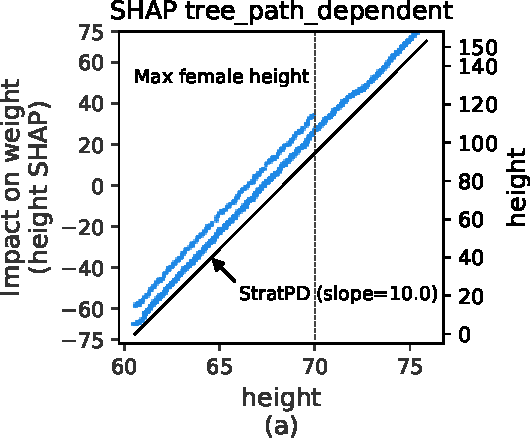
\includegraphics[scale=0.5]{images/weight-shap-tree_path_dependent.pdf}~~
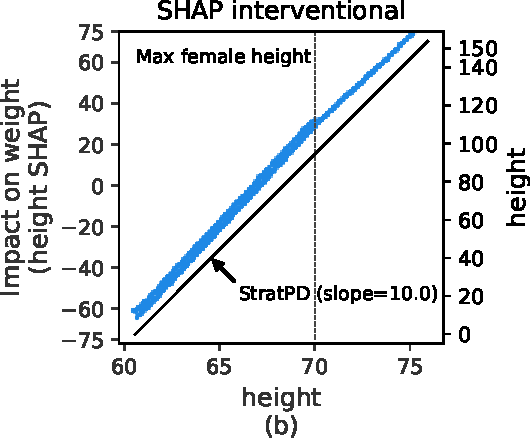
\includegraphics[scale=0.5]{images/weight-shap-interventional.pdf}
\caption{\small SHAP partial dependence plots of response body weight on feature {\tt height} using 2000 synthetic observations from Equation \eqref{eq:weight}. SHAP interrogated an RF with 40 trees and explained all 2000 samples; the interventional case used 100 observations as background data.}
\label{fig:shap-weight}
\end{center}
\end{figure}

\begin{figure}[htbp]
\begin{center}
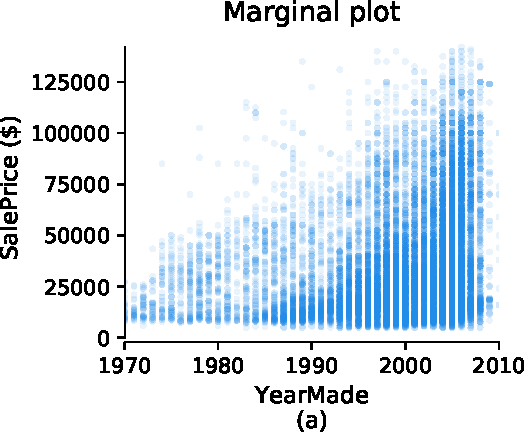
\includegraphics[scale=0.5]{images/bulldozer-YearMade-marginal.pdf}~~
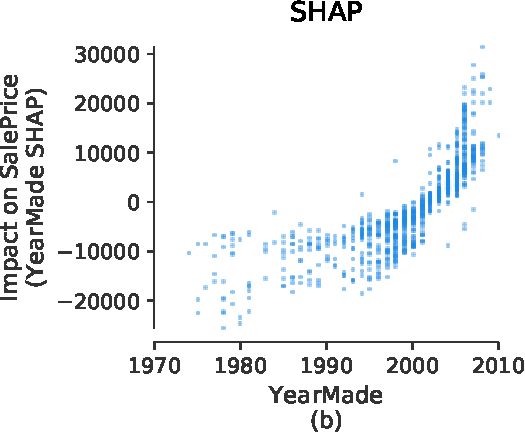
\includegraphics[scale=0.5]{images/bulldozer-YearMade-shap.pdf}~~
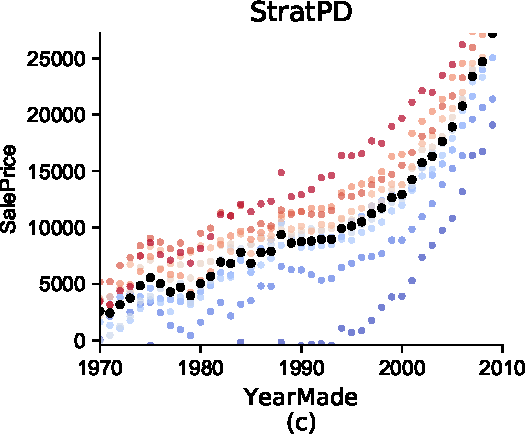
\includegraphics[scale=0.5]{images/bulldozer-YearMade-stratpd.pdf}
\caption{\small (a) Marginal plot of bulldozer {\tt YearMade} versus {\tt SalePrice} using subsample of 20k observations, (b) partial dependence drawn by SHAP interrogating an RF with 40 trees and explaining 1000 values with 100 observations as background data, (c) \spd{} partial dependence.}
\label{fig:shap-stratpd-YearMade}
\end{center}
\end{figure}

Summarize our benefits. we do not alter the data in any way. model free not just model agnostic, insensitive to codependencies, avoids having to look at subsets of features by isolating the effect of features on the response, show in the next section it is efficient. It is a simple definition and implementation based upon the stratification approach to partial dependence. 

\section{Experimental results}\label{sec:experiments}

Assessing the quality of feature impact and importance is challenging because, even with domain expertise, humans are unreliable estimators (which is why we need data analysis algorithms in the first place).  The simplest approach is to examine impacts and importances computed from synthetic data for which the answer is clear, as we did with the bodyweight data in \figref{fig:shap-weight} (impact is the area under the black line).  For real data sets, we can train a predictive model on the most impactful or most important $k$ features, as identified by the methods of interests, and then compare model prediction errors. (\citealt{mRMR} and \citealt{tsanas} also used this approach.) The method that accurately identifies the most impactful features without getting confused by codependent features, should yield lower prediction errors for a given $k$. 

In this section, we present the results of several experiments using the toy Boston data set and three real data sets, NYC rent prices \citep{rent}, bulldozer auction sales \citep{bulldozer}, and flight delays \citep{flights}. We begin with a baseline comparison of \simp{}'s importance metric to two simple model-free methods using the top-$k$ ranked features, then compare \simp{} to permutation importance and SHAP. We finish up by examining \simp's efficiency on the Kaggle data sets.

Our first experiment is to compare the feature rankings recommended by \simp{} to PCA's ranking (``loads'' associated with the first component) and to Spearman's R coefficients computed between each $x_j$ and the response variable, $y$. \figref{fig:baseline} shows mean absolute error  (MAE) versus the number of features using an RF model with 40 trees trained using the various top-$k$ feature rankings. Surprisingly, Spearman's R does a good job for all but the bulldozer data set. PCA is the opposite, performing well on bulldozer but poorly on the others. \simp{} is competitive with or surpasses these baseline techniques.  Rankings from ordinary least squares (OLS) regression coefficients, divided by their standard error, are included as a common reference curve on this and the following graphs. 

\begin{figure}
\centering
\begin{subfigure}{.245\textwidth}
    \centering
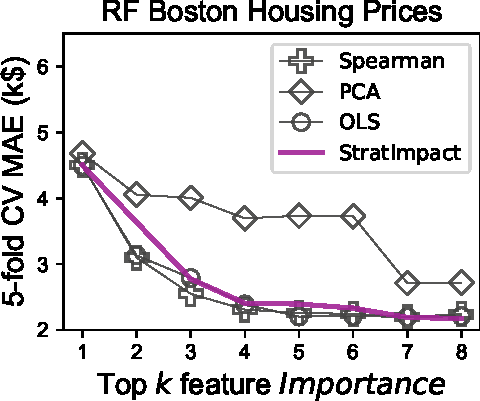
\includegraphics[scale=0.45]{images/boston-topk-baseline-Importance.pdf}
\subcaption{}
\end{subfigure}%
%\hfill
\begin{subfigure}{.245\textwidth}
    \centering
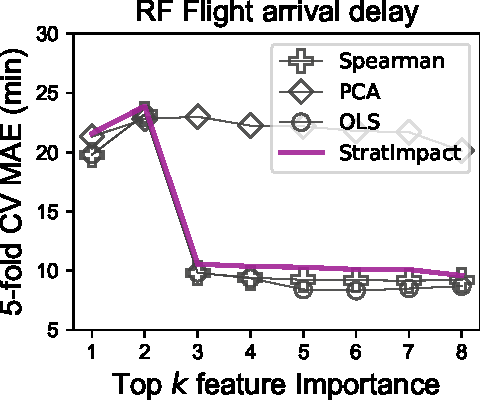
\includegraphics[scale=0.45]{images/flights-topk-baseline-Importance.pdf}
\subcaption{}
\end{subfigure}
%\hfill
\begin{subfigure}{.245\textwidth}
    \centering
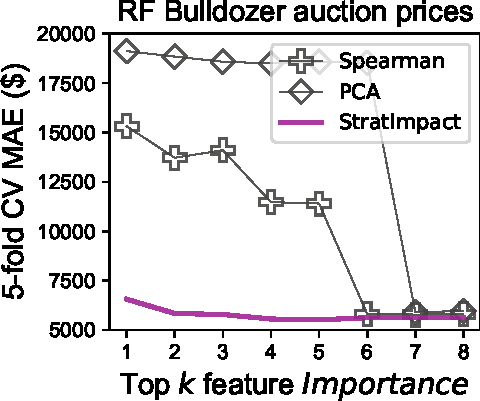
\includegraphics[scale=0.45]{images/bulldozer-topk-baseline-Importance.pdf}
\subcaption{}
\end{subfigure}
%\hfill
\begin{subfigure}{.245\textwidth}
    \centering
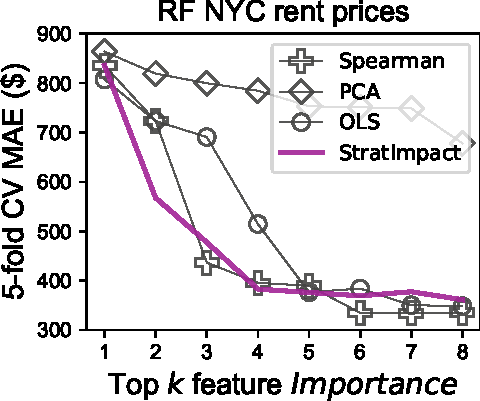
\includegraphics[scale=0.45]{images/rent-topk-baseline-Importance.pdf}
\subcaption{}
\end{subfigure} 
\caption{\small {\bf RF MAE curves from \underline{baseline} rankings}. The mean absolute error curves from 40-tree RF models trained on boston, flight, bulldozer, and rent data sets. Error curves represent 5-fold cross validation using the top-$k$ features from the following feature rankings: OLS coefficients divided by standard errors, Spearman's R between feature and response variable, PCA ``loads'' associated with the first component, and \simp{}. $n=506$ for Boston and random $n=25,000$ subsets are drawn for the other data sets. OLS used 80\% for model fitting to get coefficients, but standard errors were computed on the 20\% validation set.  Spearman's R and PCA operated on all $n$ records. \simp{} operated on just 80\% training data.}
\label{fig:baseline}
\end{figure}

Next, in \figref{fig:topk}, we compare \simp{}'s rankings to those of OLS, RF-based permutation importance, and SHAP interrogating OLS and RF models. MAE error curves were generated with an RF model trained on the top-$k$ features recommended by each technique, using $n$=25,000 records sampled from the total data set population with an 80/20 train/validation split. (Boston only has 506  total records.) RF SHAP and RF permutation importances have a distinct advantage here because they use the same kind of model (RF) for both feature ranking and top-$k$ error curves. Moreover, the model-based methods were all able to select features using the validation set, the same validation set used to compute error curves. In contrast, \simp{} cannot use predictions from a fitted model, by design, and we restricted \simp{} to examining just the training data, without access to the validation data, to see how it fared. 

\begin{figure}
\centering
\begin{subfigure}{.245\textwidth}
    \centering
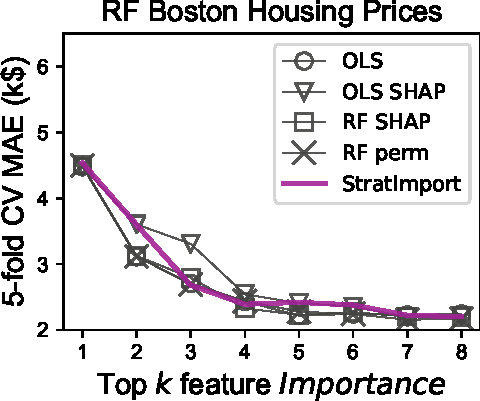
\includegraphics[scale=0.45]{images/boston-topk-RF-Importance.pdf}
\subcaption{}
\end{subfigure}%
\hfill
\begin{subfigure}{.245\textwidth}
    \centering
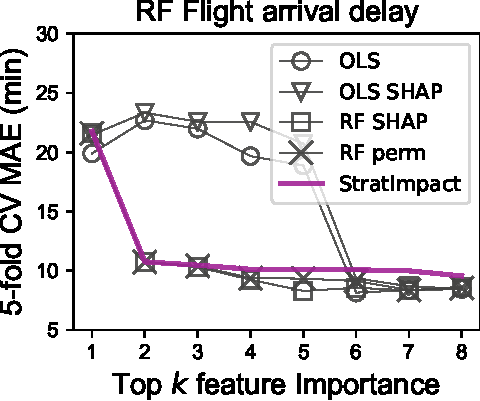
\includegraphics[scale=0.45]{images/flights-topk-RF-Importance.pdf}
\subcaption{}
\end{subfigure}
\hfill
\begin{subfigure}{.245\textwidth}
    \centering
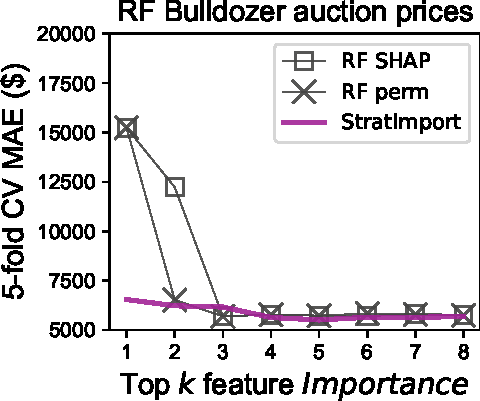
\includegraphics[scale=0.45]{images/bulldozer-topk-RF-Importance.pdf}
\subcaption{}
\end{subfigure}%
\hfill
\begin{subfigure}{.245\textwidth}
    \centering
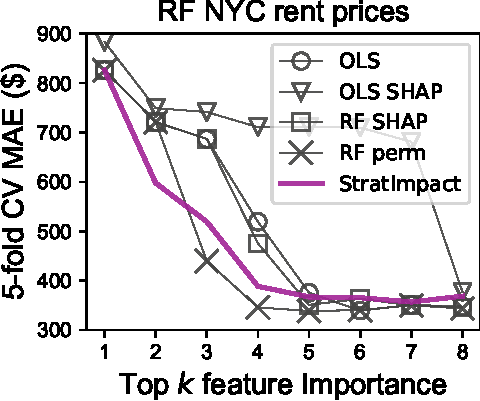
\includegraphics[scale=0.45]{images/rent-topk-RF-Importance.pdf}
\subcaption{}
\end{subfigure}
\caption[short]{\small {\bf RF MAE curves from \underline{importance} rankings}. The mean absolute error curves from 40-tree RF models trained on boston, flight, bulldozer, and rent data sets. Error curves represent 5-fold cross validation using the top-$k$ features from the following feature rankings: OLS as in \figref{fig:baseline}, SHAP interrogating OLS, SHAP interrogating 40-tree RF, permutation importance interrogating 40-tree RF, and \simp{}. All methods had access to 80\% training data from $n=25,000$ random sample (Boston has just 506 records).  All methods but \simp{} had access to the 20\% validation set.}
\label{fig:topk}
\end{figure}

Despite these handicaps, \figref{fig:topk} shows that \simp{}'s feature importances are competitive with the rankings from the other methods  applied to the four data sets.   The exception is that the \simp{} bulldozer error curve starts out higher than RF SHAP and RF permutation importance. This is because \simp{} chooses feature {\tt YearMade} as the single most important feature, whereas the RF-based techniques choose ordinal feature {\tt ProductSize}. The \simp{} bulldozer error curve then quickly converges with the RF-based curves.  Depending on the subset drawn from the various overall data set populations, the recommended rankings and error curves can shift.

The feature rankings derived from OLS perform poorly for the first few features, but then merge with the error curves from the RF-based feature rankings.  While the features were chosen by interrogating a linear model, the error curves are generated using predictions from a (stronger) RF model. Once the RF integrates sufficient numbers of features with reasonable importance, prediction error curves become more similar.  In other words, although the order might not be the best, even a linear model can provide good estimates of the top few most  predictive features. The error curve derived from the OLS SHAP feature rankings differs from the OLS curve because the OLS coefficients are divided by the standard error. Without normalizing OLS coefficients with their variances, the OLS and OLS SHAP curves merge.

\figref{fig:topk-impact} shows that the plain impact, area under the partial dependence curve unweighted by $x_j$ density, can also work well.  In the bulldozer case, for example, the first impact-ranked \simp{} feature is much better than the first \simp{} importance-ranked feature, as shown in \figref{fig:topk}(c) and \figref{fig:topk-impact}(c). (\simp{} selects the high-cardinality categorical variable {\tt ModelID}.) In fact, this impact feature yields half the MAE of all the other methods' top features. On the other hand, using impact instead of importance for the flight data set leads to a poor second rank feature choice; compare \figref{fig:topk}(b) and \figref{fig:topk-impact}(b).

\begin{figure}
\centering
\begin{subfigure}{.245\textwidth}
    \centering
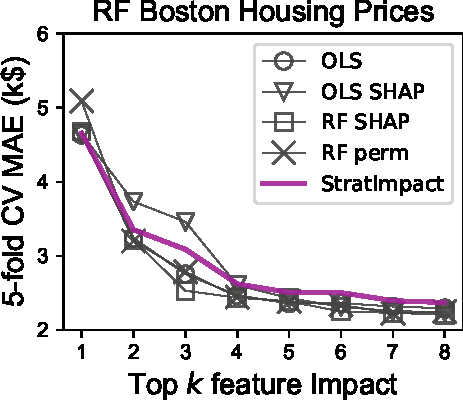
\includegraphics[scale=0.45]{images/boston-topk-RF-Impact.pdf}
\subcaption{}
\end{subfigure}%
\hfill
\begin{subfigure}{.245\textwidth}
    \centering
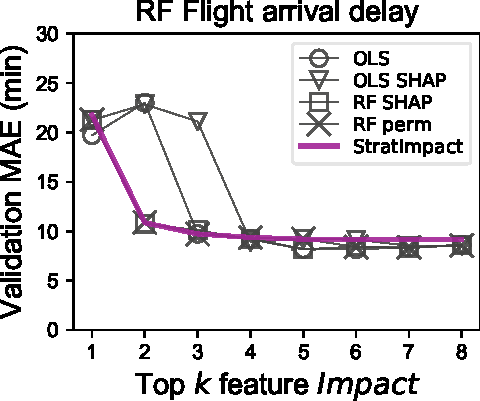
\includegraphics[scale=0.45]{images/flights-topk-RF-Impact.pdf}
\subcaption{}
\end{subfigure}
\hfill
\begin{subfigure}{.245\textwidth}
    \centering
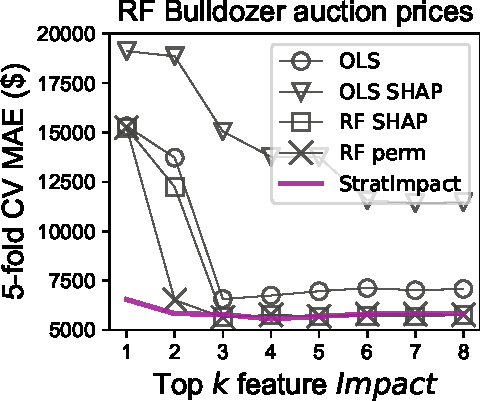
\includegraphics[scale=0.45]{images/bulldozer-topk-RF-Impact.pdf}
\subcaption{}
\end{subfigure}%
\hfill
\begin{subfigure}{.245\textwidth}
    \centering
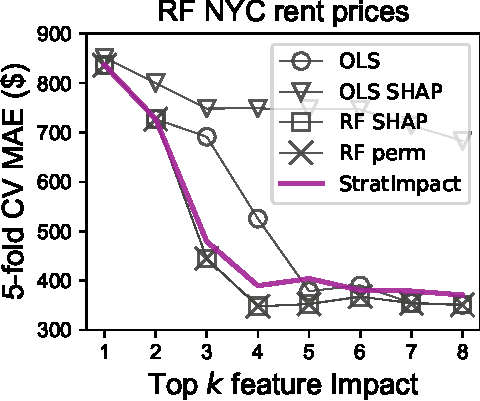
\includegraphics[scale=0.45]{images/rent-topk-RF-Impact.pdf}
\subcaption{}
\end{subfigure}
\caption[short]{\small MAE curves as in \figref{fig:topk} except using \simp{} {\em impact} rather than {\em importance}.}
\label{fig:topk-impact}
\end{figure}

Features that are predictive in one model are not necessarily predictive in another model.  To determine how well the feature rankings from the various methods ``export'' to other models, we trained gradient boosting machines (GBM) on the OLS-based, RF-based, and \simp{} feature rankings. \figref{fig:topk-gbm} shows that the \simp{} error curves generated using GBM models are similar to those resulting from RF models, except for the flight delay curve, which does not improve much after feature five while the other feature rankings do.  This could be \simp's choice of features or the fact that we used a single set of GBM hyper-parameters for all graphs, not tuning the GBMs per dataset. 

\begin{figure}
\centering
\begin{subfigure}{.245\textwidth}
    \centering
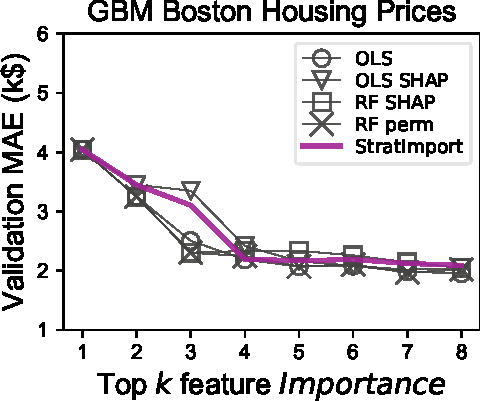
\includegraphics[scale=0.45]{images/boston-topk-GBM-Importance.pdf}
\subcaption{}
\end{subfigure}%
\hfill
\begin{subfigure}{.245\textwidth}
    \centering
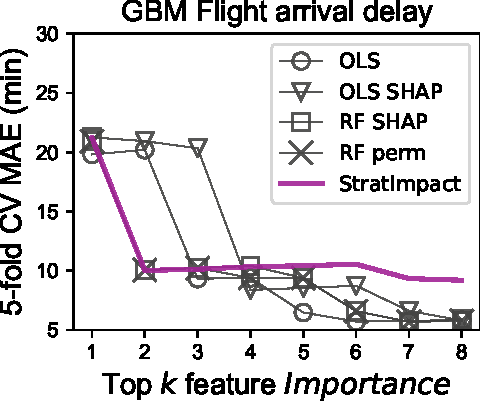
\includegraphics[scale=0.45]{images/flights-topk-GBM-Importance.pdf}
\subcaption{}
\end{subfigure}
\hfill
\begin{subfigure}{.245\textwidth}
    \centering
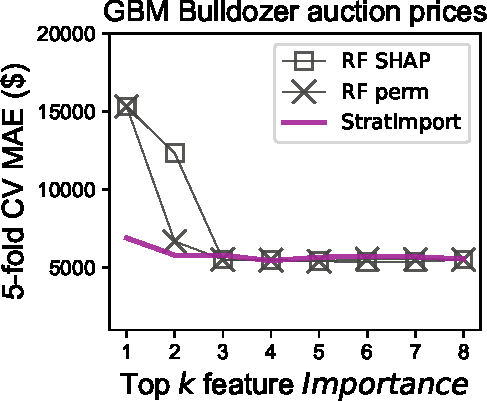
\includegraphics[scale=0.45]{images/bulldozer-topk-GBM-Importance.pdf}
\subcaption{}
\end{subfigure}%
\hfill
\begin{subfigure}{.245\textwidth}
    \centering
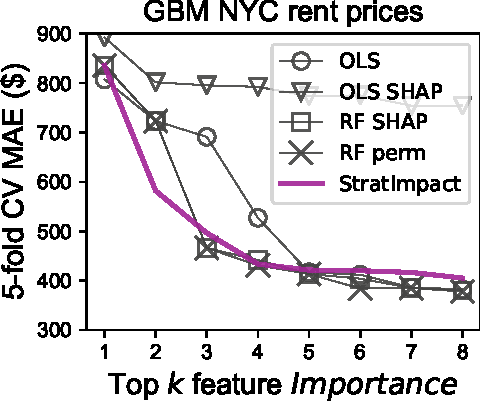
\includegraphics[scale=0.45]{images/rent-topk-GBM-Importance.pdf}
\end{subfigure}
\caption[short]{\small MAE curves as in \figref{fig:topk} except measuring {\tt xgboost} predictions, rather than RF, with learning rate 0.5,  max depth 5, and 100 trees.}
\label{fig:topk-gbm}
\end{figure}

Because GBMs are based upon decision trees (stumps) like random forests, the RF-based feature rankings would likely export well to GBM models.  To check feature exportation to a very different model, we computed error curves for the Boston and rent  data sets using OLS regressors, as shown in \figref{fig:OLS}, again using the \simp{}, OLS, and RF-derived rankings. (The Boston and rent data sets are the only ones without categorical variables, and we wanted to avoid creating tens of thousands of dummy variables for the flight and bulldozer data sets.) The error curves derived from OLS model predictions are all higher than those from RFs, as expected, but no technique's feature ranking fails to export.

We have argued that feature importance rankings derived from FPDs are the same as those derived from SHAP if the SHAP implementation approximates $\hat{f}_j(x)$ with $\Ex[\hat{f}(x_j,{\bf X}_{\bar{j}})]$, which assumes feature independence. \figref{fig:FPD_vs_SHAP} demonstrates this using the rent and bulldozer data sets. The rank and magnitude of the feature importances are extremely similar between the techniques for all $p$ features (top 8 shown here).

\begin{figure}[htbp]
\begin{center}
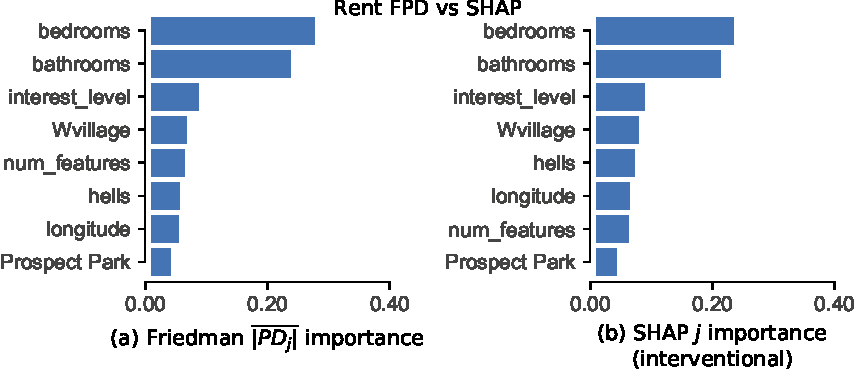
\includegraphics[scale=0.53]{images/rent-pdp-vs-shap.pdf}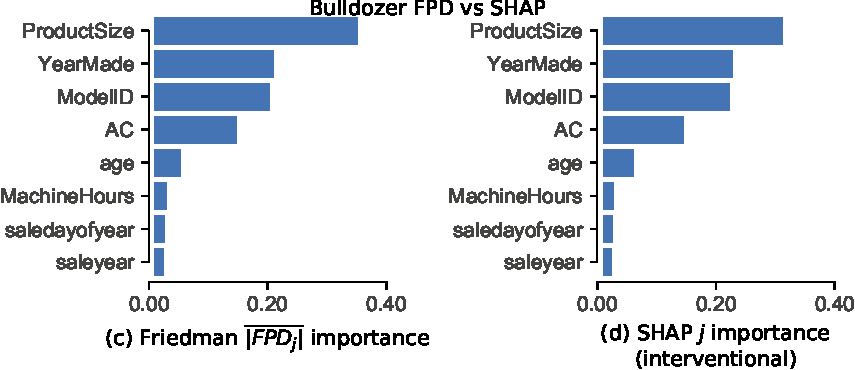
\includegraphics[scale=0.53]{images/bulldozer-pdp-vs-shap.pdf}
\caption[short]{\small  Feature importance ranking of top 8 for rent and bulldozer data sets demonstrating similarity between average magnitude of Friedman's partial dependence curves, (a) \& (c), and average magnitude of SHAP values, (b) \& (d).}
\label{fig:FPD_vs_SHAP}
\end{center}
\end{figure}

\begin{figure}[htbp]
\begin{center}
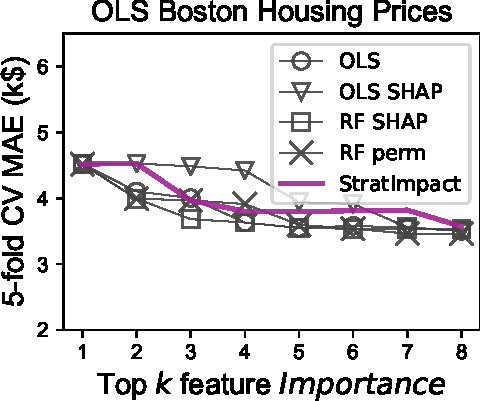
\includegraphics[scale=0.5]{images/boston-topk-OLS-Importance.pdf}~~~
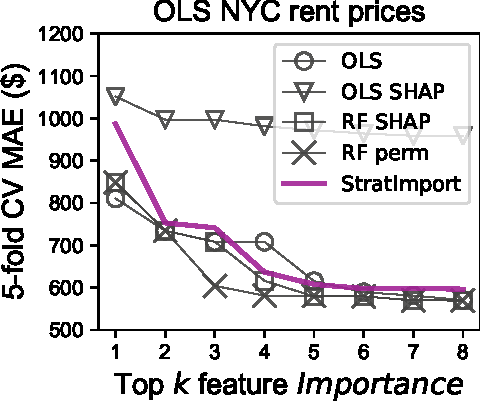
\includegraphics[scale=0.5]{images/rent-topk-OLS-Importance.pdf}
\caption[short]{\small MAE curves as in \figref{fig:topk} except measuring OLS predictions, rather than RF.}
\label{fig:OLS}
\end{center}
\end{figure}

To compute the feature rankings described thus far, we set the random seed to 1 before each test in order to get reproducible figures; computing feature impacts and importances always returns the same result for the same data as there are no random processes involved.  But, different subsets of the data set can yield very different impacts, depending on the variability of the data set. \simp{} supports subsampling with multiple trials on the overall data set to get impact standard deviations.  As an example, \figref{fig:stability} shows the  feature rankings from \simp{} importance and impact, averaged from 10 trials using 75\% subsamples selected randomly from the 48k records of the rent data set. The error bars show two standard deviations (a red error bar indicates it reaches 0). The high variances of the neighborhood features, such as {\tt UpperEast} and {\tt astoria}, arise because those features represent the $L_1$ distance from each apartment's longitude/latitude to that neighborhood. The distance-to-neighborhood features have similar importance and selection depends on vagaries of the data set.
 
\begin{figure}[htbp]
\begin{center}
\begin{subfigure}{.45\textwidth}
    \centering
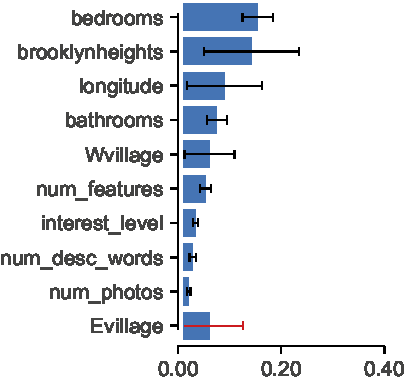
\includegraphics[scale=0.65]{images/rent-stability-importance.pdf}
\subcaption{\simp{} Rent Importance}
\end{subfigure}%
\begin{subfigure}{.45\textwidth}
    \centering
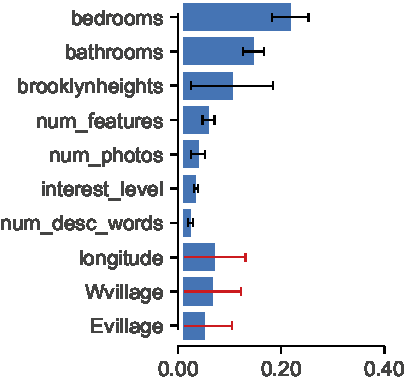
\includegraphics[scale=0.65]{images/rent-stability-impact.pdf}
\subcaption{\simp{} Rent Impact}
\end{subfigure}%
\captionof{figure}{\small  Average feature importance and impact across 10 trials on the rent data set, with 75\% subsamples from 48k total records.  Error bars show two standard deviations; red indicates two standard deviations reach zero.}
\label{fig:stability}
\end{center}
\end{figure}

Because we are primarily concerned with computing variable impacts to gain business and medical insights, speed is less of a concern---practitioners would likely run \simp{} on their entire data set once, or at least much less often than techniques for feature selection during modeling. (Feature selection, must be more performant as practitioners need to iterate quickly when developing models.)   Nonetheless, it is worthwhile analyzing \simp{} time complexity and demonstrating that it operates in a reasonable amount of time empirically.

The cost of computing each $x_j$'s impact is dominated by the cost of computing the partial dependence and a pass over the unique $x_j$ values to compute the mean. Computing the importance costs an extra pass over all $n$ $x_j$ values to get the histogram. The upper bound  complexity for \spd{} and \cspd{} partial dependences is $O(n \times |unique(x_j)|)$, or just $O(n^2)$ in the worst case.   Because $|unique(x_j)|$ is usually much smaller than $n$ in real data sets, \spd{} typically performs linearly, but \cspd{} exhibits quadratic behavior.  The overall worst case behavior for \simp{} is then $p \times (|unique(x_j)| + n^2)$ to get $p$ impacts and $p \times (n + |unique(x_j)| + n^2)$  to get $p$ importances, giving asymptotic behavior of $O(n^2)$.

\begin{figure}
\centering
\begin{tabular}{r r r r r r r r r}
{\bf dataset} & $p$ & catvars & {\small $n$=1,000} & {\small 10,000} & {\small 20,000} & {\small 30,000} & time versus $n$~~ & $R^2$\\
\hline
{\tt\small flight} & 17 & 5 & 0.6s & 18.4s & 65.4s & 152.7s & {\small $-0.219 n + 0.170 n^2$} & {\small 0.9990}\\
{\tt\small bulldozer} & 14 & 2 & 0.2s & 2.7s & 8.6s & 18.3s & {\small $0.078 n + 0.017 n^2$} & {\small 0.9997}\\
{\tt\small rent} & 20 & 0 & 0.3s & 3.7s & 8.2s & 13.0s & {\small $0.385 n + 0.002 n^2$} & {\small 0.9985}\\
\end{tabular}
\caption{\small  Execution time for subsets of size 1,000 to 30,000 stepping by 1,000 43 real data sets. Rent has no categorical variables and exhibits linear performance, whereas categorical variables introduce mildly quadratic behavior. Final two columns describe how data fits to quadratic equations.}
\label{fig:timing}
\end{figure}

In practice, importances for numerical variables are nearly linear and importances for categorical variables are mildly quadratic. \figref{fig:timing} summarizes the empirical time in seconds to compute importances for a range of subset sizes for the three Kaggle data sets. The ``time versus $n$'' and $R^2$ columns describe a quadratic fit to the curve representing the time (in seconds) required to compute subsets from $n=1$ to 30,000 stepping by 1,000. The rent data set has no categorical variables and grows linearly with $n$, possibly with a small quadratic component. The flight data set, on the other hand, shows clear quadratic behavior due to the (five) categorical variables. Despite the highly nonlinear worst-case complexity, \figref{fig:timing} suggests our Python-only \simp{} prototype is fast enough for use on real data sets of sizes in the tens of thousands. 

\cut{
cost of \spd{} is cost to train RF then cost to walk leaves and perform piecewise linear approximation for each leaf. Then average the slope-ranges.  piecewise linear approximation is a function of elements in leaf but in total, we are computing differences on all n elements. to average the slopes together, it's a function of how many slopes, which could be n If all values are unique. There are roughly unique x by n slopes in a matrix of values that we collapse to get average slope in a range.  Integrating the slopes, the partial derivatives, is O(unique x). 
Bulldozer:
X.shape=(362781, 14)
uniq x = 5 slopes.shape = (8112,) x ranges.shape (8112, 2)
uniq x = 59 slopes.shape = (8242,) x ranges.shape (8242, 2)
uniq x = 22 slopes.shape = (10145,) x ranges.shape (10145, 2)
uniq x = 10887 slopes.shape = (23200,) x ranges.shape (23200, 2)
uniq x = 59 slopes.shape = (8587,) x ranges.shape (8587, 2)
uniq x = 6 slopes.shape = (2641,) x ranges.shape (2641, 2)
uniq x = 2 slopes.shape = (3265,) x ranges.shape (3265, 2)
uniq x = 2 slopes.shape = (3177,) x ranges.shape (3177, 2)
uniq x = 12 slopes.shape = (15967,) x ranges.shape (15967, 2)
uniq x = 31 slopes.shape = (28357,) x ranges.shape (28357, 2)
uniq x = 7 slopes.shape = (11874,) x ranges.shape (11874, 2)
uniq x = 293 slopes.shape = (32103,) x ranges.shape (32103, 2)
Impact importance time 61s

Rent:
X.shape=(48299, 20)
uniq x = 8 slopes.shape = (3436,) x ranges.shape (3436, 2)
uniq x = 9 slopes.shape = (1027,) x ranges.shape (1027, 2)
uniq x = 1933 slopes.shape = (11814,) x ranges.shape (11814, 2)
uniq x = 1364 slopes.shape = (11759,) x ranges.shape (11759, 2)
uniq x = 3 slopes.shape = (2139,) x ranges.shape (2139, 2)
uniq x = 3374 slopes.shape = (12159,) x ranges.shape (12159, 2)
uniq x = 4091 slopes.shape = (12098,) x ranges.shape (12098, 2)
uniq x = 4585 slopes.shape = (12034,) x ranges.shape (12034, 2)
uniq x = 4452 slopes.shape = (11968,) x ranges.shape (11968, 2)
uniq x = 4506 slopes.shape = (12020,) x ranges.shape (12020, 2)
uniq x = 4473 slopes.shape = (12088,) x ranges.shape (12088, 2)
uniq x = 4194 slopes.shape = (12029,) x ranges.shape (12029, 2)
uniq x = 3141 slopes.shape = (12003,) x ranges.shape (12003, 2)
uniq x = 3440 slopes.shape = (11996,) x ranges.shape (11996, 2)
uniq x = 4234 slopes.shape = (12005,) x ranges.shape (12005, 2)
uniq x = 4389 slopes.shape = (12089,) x ranges.shape (12089, 2)
uniq x = 3598 slopes.shape = (12082,) x ranges.shape (12082, 2)
uniq x = 42 slopes.shape = (8551,) x ranges.shape (8551, 2)
uniq x = 355 slopes.shape = (16019,) x ranges.shape (16019, 2)
uniq x = 29 slopes.shape = (9204,) x ranges.shape (9204, 2)
Impact importance time 13s

flight has 5,819,080 records.
}



The entire \simp{} code base is available at {\tt\small https://github.com/parrt/stratx} and running {\tt\small articles/imp/genfigs/RUNME.py} will regenerate all figures in this paper, after downloading the three Kaggle data sets.  Simulations were run on a 4.0 Ghz 32G RAM machine running OS X 10.13.6 with SHAP 0.34, scikit-learn                       0.21.3, XGBoost 0.90, and Python 3.7.4.

\section{Discussion and future work}\label{sec:discussion}

In this paper, we propose a model-free approach for measuring feature $x_j$'s true impact upon the response variable, $y$, based upon a mathematical definition of impact that is a function of $x_j$'s partial dependence curve. By weighting $x_j$'s partial dependence curve with $x_j$'s density, we also arrive at a mathematical definition of feature importance.   In contrast, most existing techniques and research focus on model feature selection, through a plurality of feature importance definitions.   The exception is SHAP, which provides a mathematical definition of feature impact, though based upon predictions from a fitted model, rather than directly from the data.

The focus on feature selection is understandable because practitioners commonly incorporate feature selection into the model development cycle in an effort to simplify models. For this purpose, though, only relative feature ranks matter, not the specific importance values {\em per se}.  For example, permutation importance  computes model prediction accuracy differences from the full baseline model, which are related to but not the same as feature impacts. Many (model-free) techniques, such as mRMR, provide just a ranking, without specific importance values.

Obtaining feature importance through impact is valid because the most impactful features should be the most predictive in a variety of models, but the opposite is not the case.   Interpreting importances as feature impacts is inappropriate because predictive features does not always coincide with impactful features.  The same importance technique applied to the same data can get very different feature importances, depending on the model, which calls into question their validity as impact values.  Feature impacts, and hence business and medical insights, should be derived directly from the data, not through the lens of a model.

To assess the quality of \simp's feature impacts, we compared \simp's recommended feature importance rankings to those of other techniques, as a proxy, in the previous section. Despite not having access to predictions from a fitted model nor the 20\% validation set, \simp{} feature rankings are competitive for three real data sets. We conclude that \simp{} is a promising approach for obtaining feature impacts.  

As for model feature selection, the bulldozer error curves in \figref{fig:topk-impact}(c) illustrate a case where \simp{} (ranked by impact not importance) gets half the error rate of the top features recommended by the other methods.  One would expect model-based techniques to easily identify the single most important model feature, or at least more readily than a model-free approach.  (\simp{} recommends the high-cardinality categorical variable {\tt ModelID}, whereas RF-based permutation importance and SHAP recommend ordinal {\tt ProductSize}.)  Even if such results are rare, misidentifying the single most important feature indicates that there is room for improvement in the feature importance research area. 

It is also interesting to note that simple expedients like ranking features by Spearman's R coefficient between $x_j$ and $y$ or simple techniques like permutation importance perform well, at least for the first eight important features in our experiments. (We did not perform experiments on the least important features.) Also note that the error curves for SHAP and permutation importance generally mirror each other for the first eight features.  Both techniques introduce potentially nonsensical records to avoid retraining models, but this does not appear to affect their ability to rank features for feature selection purposes.

The best-performing feature selection techniques are typically expensive, depending on the data subsets size and model used (in the model-based case).  \simp{} has $O(n^2)$ asymptotic complexity but exhibits linear performance for numerical and mildly-quadratic behavior for categorical variables on the three real data sets tested here.  The execution time of the \simp{} prototype is satisfactory in our experiments, though the flight data set takes 2.5 minutes to analyze 30,000 records (compared to 13 seconds for the rent data set that does not have categorical variables).

Each of the $p$ feature $x_j$ impact computations is independent and could proceed in parallel. Unfortunately, our casual attempts at parallelizing the algorithm across multiple CPU cores was thwarted by Python's dreaded ``global interpreter lock'' (threading) or passing data between processes (process-based threading).  We did, however, get increased performance using the Numba just-in-time compiler ({\tt\small http://numba.pydata.org}) on algorithm hotspots (at the cost of 5 seconds of compiler warmup time at runtime). Reimplementation in C would be the next step and should dramatically increase performance over the pure-Python prototype.

The \simp{} approach relies on accurate partial dependences for both numerical and categorical variables, and considerable effort has gone into refining the current partial dependence algorithms. Extensive simulation has shown, however, that partial dependences computed using the stratification approach are highly sensitive to partial derivatives computed for the left edge of any $x_j$'s range. The partial dependence curve is the cumulative sum of the partial derivatives and so any changes at the left edge affect the entire curve.  This presents a problem when there are few samples with $x_j$ values in that range, as shown in the histogram of \figref{fig:yearmade}. (We introduced a hyper-parameter called {\tt\small min\_slopes\_per\_x\_values} to ignore any partial derivatives estimated with too few records, which improved the accuracy and stability of the partial dependence estimates.)  Any improvement in partial dependence curves would be useful in their own right and particularly helpful for \simp.    Another key area of improvement would be partial dependences for classification data sets, since \simp{} cannot compute impacts for classifiers until such partial dependences are available.


\appendix

\section{Proof relating SHAP values and partial dependence curves}

The shapley regression values for features $F=\{1,..,p\}$ per \cite{shap} are as follows, simplifying the weight term and using model $\hat{f}$.

\begin{equation}\label{shapregr}
\phi_j(\hat{f},x) = \sum_{S \subseteq F \texttt{\char`\\} \{j\}}\
%\frac{|S|!(|F|-|S|-1)!}{|F|!}\
\frac{1}{p{{p-1}\choose{|S|}}}\
 [ \hat{f}_{S \cup \{j\}}(x_{S \cup \{j\}}) - \hat{f}_S(x_S) ]
\end{equation}

The contribution of feature $j$ is the weighted average difference between $\hat{f}(x)$ for $x$ with and without $j$, $\hat{f}(x_{S \cup \{j\}}) - \hat{f}(x_S)$. SHAP approximates the model trained on just $S$ features, $\hat{f}_S(x_S)$, with $\Ex[\hat{f}(x_{S},{\bf X}_{\bar{S}}) | {\bf X}_S = x_S]$ then further approximates with $\Ex[\hat{f}(x_{S},{\bf X}_{\bar{S}})]$ by assuming independent features. \cite{janzing2019feature} argues that $\Ex[\hat{f}(x_{S},{\bf X}_{\overline{S}})]$ is ``... conceptually the right thing in the first place.'' \todo{that stuff is repeat} To show the relationship between SHAP values and traditional FPD partial dependence curves, as defined by \cite{PDP}, we state and prove the following theorem.

\begin{theorem}
The average of the SHAP values at any $x_j=z$ location estimates the mean-centered FPD partial dependence curve, assuming independent features: $\Ex[ \phi_j(\hat{f},x) | {\bf X}_j = z] = FPD_j(x) - \bar{y}$.
\end{theorem}

\begin{proof}
{\em Part 1: } Show $\phi_j(\hat{f},x)$ is the difference between $\hat{f}(x)$ and the FPD curve, as defined by Friedman, for features $F \texttt{\char`\\} \{j\}$ (all features except $j$). For independent features, we can choose any subset $S \subseteq F \texttt{\char`\\} \{j\}$ to measure the impact of feature $j$, therefore, we choose $S = F \texttt{\char`\\} \{j\}$. Since ${{p-1}\choose{|S|}} = {{p-1}\choose{p-1}} = 1$, the weight reduces to $1/p$:

\[
\phi_j(\hat{f},x) = \sum_{S \subseteq F \texttt{\char`\\} \{j\}}\
%\frac{|S|!(|F|-|S|-1)!}{|F|!}\
\frac{1}{p}\
 [ \hat{f}_{S \cup \{j\}}(x_{S \cup \{j\}}) - \hat{f}_S(x_S) ]
\]

\noindent Replace $\hat{f}_S(x_{S})$ by $\Ex[\hat{f}(x_{S},{\bf X}_{\bar{S}})]$ and, because $S$ is fixed, remove the summation:

\[
\phi_j(\hat{f},x) = \frac{1}{p}\
 ( \Ex[\hat{f}(x_{S \cup \{j\}},{\bf X}_{\overline{S \cup \{j\}}})] - \Ex[\hat{f}(x_{S},{\bf X}_{\bar{S}})] )
\]

\todo{ah ha! 1/p goes away because it is counting the number of permutations but we are only using one}

\noindent Per {\tt\small bruteforce.py}\footnote{\tt https://github.com/slundberg/shap/blob/master/shap/explainers/bruteforce.py} in the SHAP codebase and Equation 11 in \cite{shap}, SHAP approximates the marginal expectation, assuming feature independence, as:

\[
\Ex[\hat{f}(x_{S},{\bf X}_{\bar{S}})] = \
    \frac{1}{n} \sum_{i=1}^n \hat{f}(x_S, x_{\bar{S}}^{(i)})
\]

\noindent But, that summation is equivalent to the approximation of $j$'s partial dependence curve (Equation 53 in \citealt{PDP}), giving:

\[
\phi_j(\hat{f},x) = \frac{1}{p}\
(  \text{\it FPD}_{S \cup \{j\}}(x) - \text{\it FPD}_{S}(x) )
\]

\noindent or, since $S = F \texttt{\char`\\} \{j\}$:

\[
\phi_j(\hat{f},x) = \frac{1}{p}\
(\text{\it FPD}_{F}(x) - \text{\it FPD}_{F \texttt{\char`\\} \{j\}}(x))
\]

\cut{
$\phi_j$ is, therefore, the difference between points on two partial dependence curves, one curve derived using $F$, which is just $\hat{f}(x)$, and one derived from $F \texttt{\char`\\} \{j\}$. 
}

\noindent  Because $\text{\it FPD}_{F}(x) = \hat{f}_F(x_F) = \hat{f}(x)$, the equation simplifies to the difference between $\hat{f}(x)$ and the marginal effect of $j$ at point $x$:

\[
\phi_j(\hat{f},x) = \frac{1}{p}( \hat{f}(x) - \text{\it FPD}_{F \texttt{\char`\\} \{j\}}(x) )
\]

\todo{Since $\frac{1}{p}$ is common to all features it's tempting to take it out, but it affects the Shapley value in the math so it seems like we should keep it in.  I verified that mean(abs(Friedman FPD)) is same as avg abs SHAP values so clearly that constant goes away somehow. it must have something to do with the $\bar{y}$ that is subtracted to get the mean centered version.} 

\noindent {\em Part 2}. Show that the expected SHAP value at a specific $x_j=z$ value is a point on the mean-centered FPD curve:


\[
\Ex[ \phi_j(\hat{f},x) | {\bf X}_j = z] = \text{\it FPD}_j(x) - \bar{y}
\]

\noindent Take the expected value of $\phi_j(\hat{f},x)$ conditioned on each instance in $\bf X$ using value $z$ for feature $j$:

\[
\Ex[ \phi_j(\hat{f},x) | {\bf X}_j = z ] = \Ex [\hat{f}(x) | {\bf X}_j = z ] - \Ex [ \text{\it FPD}_{F \texttt{\char`\\} \{j\}}(x) | {\bf X}_j = z ]
\]

\noindent $\Ex [\hat{f}(x) | {\bf X}_j = z ]$ is the expected value across all $\bf X$ with a fixed $x_j=z$ value taken from $x$, which is the definition of $FPD_j(x)$:

\[
\Ex[ \phi_j(\hat{f},x) | {\bf X}_j = z ] = FPD_j(x) - \Ex [ \text{\it FPD}_{F \texttt{\char`\\} \{j\}}(x) | {\bf X}_j = z ]
\]

\noindent $\text{\it FPD}_{F \texttt{\char`\\} \{j\}}(x)$  fixes $F \texttt{\char`\\} \{j\}$ and the conditional ${\bf X}_j = z$ fixes $j$, yielding 

\[
\Ex[ \phi_j(\hat{f},x) | {\bf X}_j = z ] = FPD_j(x) - \Ex_{\bf X} [ \text{\it FPD}_{F}(x) ]
\]

\todo{That conversion from conditional expectation to $\Ex_{\bf X}$ seems a bit off to me in the last step.}

\noindent Since, $\text{\it FPD}_{F}(x) = \hat{f}(x)$:

\[
\Ex[ \phi_j(\hat{f},x) | {\bf X}_j = z ] = FPD_j(x) - \Ex_{\bf X} [ \hat{f}(x) ] = FPD_j(x) - \bar{y}
\]

\noindent which completes the proof.

\end{proof}


% -----------
\cut{
$\Ex_{\bf X} [\hat{f}(x)]$ is just $\overline{\hat{f}({\bf X})} = \bar{y}$ and $\text{\it PDP}_{F \texttt{\char`\\} \{j\}}(x)$ is equivalent to $ICE_j(x)$, the Individual Conditional Expectation ({\em ICE}) from \cite{ice}, which simplifies the equation to: 

\[
\Ex_{\bf X}[ \phi_j(\hat{f},x) ] = \bar{y} - \Ex_{\bf X}[ ICE_j(x) ]
\]

\noindent By definition, $PDP_j(x) = \Ex_{\bf X}[ ICE_j(x) ]$, the PDP curve is the average of all ICE curves derived from $x \in {\bf X}$:

\cut{
\[
\Ex_{\bf X}[ \phi_j(\hat{f},x) ] = \bar{y} - \frac{1}{n} \sum_{i=1}^n ICE_j(x^{(i)})
\]
}

\[
\Ex_{\bf X}[ \phi_j(\hat{f},x) ] = \bar{y} - \text{\it PDP}_j(x)
\]

The shap values are not directly on the PDP curve but their average is:

\[
\text{\it PDP}_j(x) = \bar{y} - \Ex_{\bf X}[ \phi_j(\hat{f},x) ]
\]

\todo{ seems like it should be $\Ex_{\bf X}[ \phi_j(\hat{f},x) ] - \bar{y}$, with the flipped sign. also, maybe it needs to be conditioned:}

\[
\text{\it PDP}_j(x) = \bar{y} - \Ex[ \phi_j(\hat{f},x) | {\bf X}_j = x_j]
\]

Try alternative approach, which is to expand everything out:

\[
\Ex_{\bf X}[ \phi_j(\hat{f},x) ] = \frac{1}{n} \sum_{k=1}^n \hat{f}(x^{(k)}) - \
\frac{1}{n} \sum_{k=1}^n \Ex_{\bf X}[ \text{\it PDP}_{F \texttt{\char`\\} \{j\}}(x) ]
\]

\[
\Ex_{\bf X}[ \phi_j(\hat{f},x) ] = \bar{y} - \
\frac{1}{n} \sum_{k=1}^n \frac{1}{n} \sum_{i=1}^n \hat{f}(x_{F \texttt{\char`\\} \{j\}}^{(k)}, x_j^{(i)})
\]

 Reorder the summations:
 
\[
\Ex_{\bf X}[ \phi_j(\hat{f},x) ] = \bar{y} - \
\frac{1}{n} \sum_{i=1}^n \frac{1}{n} \sum_{k=1}^n  \hat{f}(x_{F \texttt{\char`\\} \{j\}}^{(k)}, x_j^{(i)})
\]

Then

\[
\Ex_{\bf X}[ \phi_j(\hat{f},x) ] = \bar{y} - \
\frac{1}{n} \sum_{i=1}^n \text{\it PDP}_j(x^{(i)})
\]

The expected value of any PDP curve is $\hat{y}$ since the total of all $PDP_j(x)$ curves is $\hat{f}(x)$; divide by $n$ and we get $\bar{y}$. So:

\[
\Ex_{\bf X}[ \phi_j(\hat{f},x) ] = \bar{y} - \bar{y} = 0
\] 

\todo{ it makes sense that the expected value of the Shapley curve is 0 but I'm not sure that proves it's a mean centered PDP. lots of things could equal zero.}


The impact of $j$ on $y$ is the average $\phi_j(\hat{f},x^{(i)})$ magnitude:

\[
\frac{1}{n} \sum_{i=1}^n |  \hat{f}(x^{(i)}) - \text{\it PDP}_{F \texttt{\char`\\} \{j\}}(x^{(i)}) |
\]

 it doesn't follow but do we want to extract out $\bar{y}$?
 
\[
\frac{1}{n} \sum_{i=1}^n \hat{f}(x^{(i)}) - \frac{1}{n} \sum_{i=1}^n \text{\it PDP}_{F \texttt{\char`\\} \{j\}}(x^{(i)})
\]

\[
\overline{\hat{f}({\bf X})} - \frac{1}{n} \sum_{i=1}^n \text{\it PDP}_{F \texttt{\char`\\} \{j\}}(x^{(i)})
\]
}


\cut{
\noindent since $S = F \texttt{\char`\\} \{j\}$:

\[
\phi_j(\hat{f},x) = \frac{1}{p}\
 [ \Ex[\hat{f}(x_F,{\bf X}_\emptyset)] - \Ex[\hat{f}(x_{F \texttt{\char`\\} \{j\}},{\bf X}_{j})] ]
\]

Janzing says ``We now want to attribute the difference between f(x) and the expectation E[f(X)] to individual features.''


The code in {\tt\small bruteforce.py}\footnote{\tt https://github.com/slundberg/shap/blob/master/shap/explainers/bruteforce.py} has a simple but inefficient implementation that computes $\phi$ values using  {\tt\small f\_without\_j}, which is $PDP_S(x)$ ($i$ changed to $j$ to be consistent with our notation):

{\small
\begin{verbatim}
masker = lambda x, mask: x * mask + masker_data * np.invert(mask)
mask[list(S)] = 1
f_without_j = f(masker(x, mask)).mean(0)
mask[j] = 1
f_with_j = f(masker(x, mask)).mean(0)
phi[j,:] += weight * (f_with_j - f_without_j)
\end{verbatim}}

}


\cut{
\begin{figure}
\centering
\begin{subfigure}{1\textwidth}
    \centering
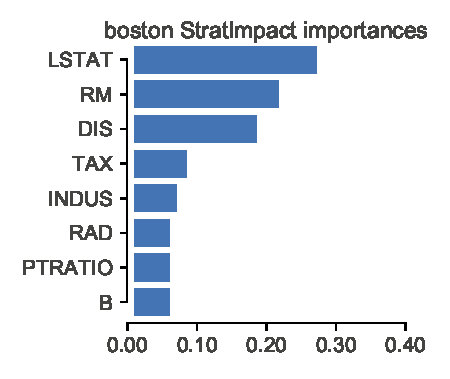
\includegraphics[scale=0.5]{images/boston-features.pdf}
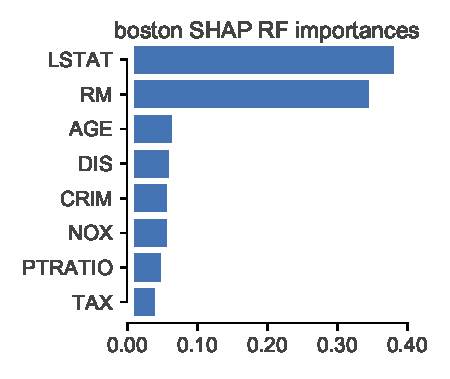
\includegraphics[scale=0.5]{images/boston-features-shap-rf.pdf}
\vspace{-2mm}\subcaption{\footnotesize Note LSTAT/RM order is diff than in original figure as their is high variance}\vspace{3mm}
\end{subfigure}%
\hfill
\begin{subfigure}{1\textwidth}
    \centering
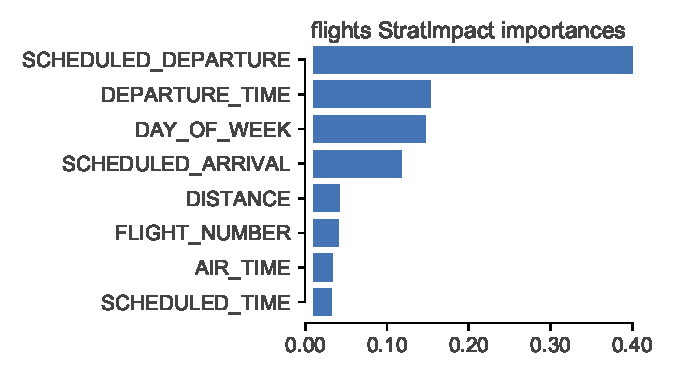
\includegraphics[scale=0.5]{images/flights-features.pdf}
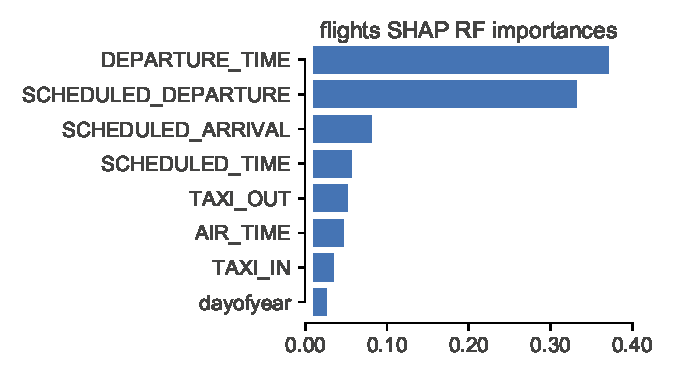
\includegraphics[scale=0.5]{images/flights-features-shap-rf.pdf}
\vspace{-2mm}\subcaption{\footnotesize 5.8M records}\vspace{3mm}
\end{subfigure}
\hfill
\begin{subfigure}{1\textwidth}
    \centering
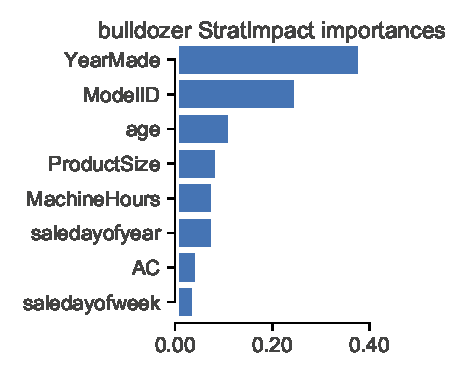
\includegraphics[scale=0.5]{images/bulldozer-features.pdf}
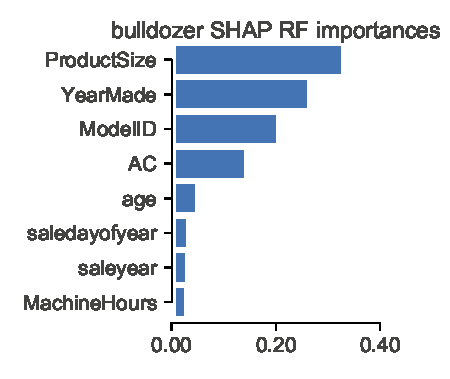
\includegraphics[scale=0.5]{images/bulldozer-features-shap-rf.pdf}
\vspace{-2mm}\subcaption{\footnotesize foo}\vspace{3mm}
\end{subfigure}%
\hfill
\begin{subfigure}{1\textwidth}
    \centering
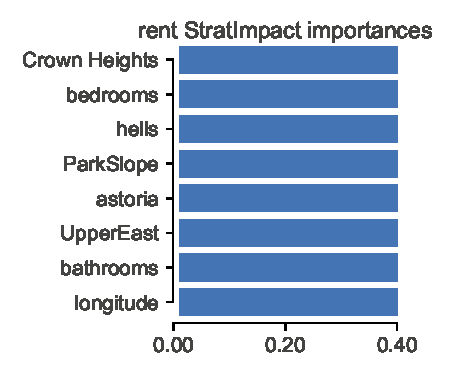
\includegraphics[scale=0.5]{images/rent-features.pdf}
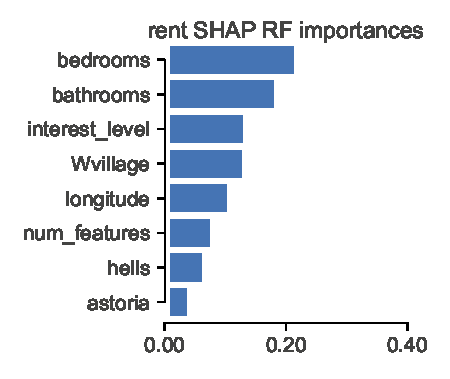
\includegraphics[scale=0.5]{images/rent-features-shap-rf.pdf}
\vspace{-2mm}\subcaption{\footnotesize foo}\vspace{3mm}
\end{subfigure}
\caption[short]{blorttttt}
\label{fig:features}
\end{figure}
}

\vskip 0.2in
\bibliography{pdimp}
\end{document}